%%============
%%  ** Author: Shepherd Qirong
%%  ** Date: 2021-12-20 22:40:58
%%  ** Github: https://github.com/ShepherdQR
%%  ** LastEditors: Shepherd Qirong
%%  ** LastEditTime: 2021-12-20 23:41:39
%%  ** Copyright (c) 2019--20xx Shepherd Qirong. All rights reserved.
%%============


\chapter{Introduction}
Today is 20211204, and I deciede to note down all of my knowledge about the math in this notebook.


\section{Space}

\subsection{Operation Defination}

\subsubsection{Element}

we define the basic element $\boldsymbol x = [x_1, x_2,\dots]^T = \Sigma x_i \boldsymbol{e_i}$, $ \boldsymbol e_i $ means $x_i = 1, x_j = 0$ for all $j \neq i$. We define Kronecker sign to simply the description of $\boldsymbol e_i \cdot \boldsymbol e_j $.

\begin{equation}
    \begin{split}
    &\delta _{i,j}:=
    \begin{cases}
    &1,\qquad i = j\\
    &0,\qquad i \neq j\\
    \end{cases}\\
    \end{split}
\end{equation}

The set of bases $\{ \boldsymbol e_i  \}  \stackrel{apply}{\longrightarrow} \boldsymbol{x} \longrightarrow    \{ x_i \}    $.




\subsubsection{Dot Product}

We define in algebra, $ \boldsymbol{x} \cdot \boldsymbol{y} := \sum{x_iy_i\boldsymbol{e}_i} = \boldsymbol{x}^T \cdot \boldsymbol{y}$.

Then the defination is restricted to the choose of the coordinate system. We take a look a the product with reflect $T : \boldsymbol x \rightarrow  \boldsymbol{T} \cdot \boldsymbol{x}$,

\begin{equation}
    (\boldsymbol A \cdot \boldsymbol  B)^T = (a_{ik}b_{kj})^T = c_{ij}^T = c_{ji} = b_{jk}a_{ki} = \boldsymbol B^T \cdot \boldsymbol A^T
\end{equation}
we have 
\begin{equation}
    (\boldsymbol T \cdot \boldsymbol  x)^T(\boldsymbol T \cdot \boldsymbol  y) =  \boldsymbol x^T (\boldsymbol T^T \boldsymbol T) \boldsymbol y = [(\boldsymbol T^T \boldsymbol T) \boldsymbol x]^T \boldsymbol y
\end{equation}

We name T a Contractive mapping when $\boldsymbol T^T \boldsymbol T \leqslant   \theta, 0 \leqslant \theta \leqslant 1$.

\subsubsection{geometry Properties}

\begin{equation}
    \begin{split}
    &\parallel \boldsymbol{x} \parallel := \sqrt{\boldsymbol x \cdot \boldsymbol x}\\
    &\cos {\theta_{x,y}} : = \frac
    {\boldsymbol x \cdot \boldsymbol x}
    {\parallel \boldsymbol{x} \parallel \cdot \parallel \boldsymbol{y} \parallel}\\
\end{split}
\end{equation}

\subsubsection{Add}

\begin{equation}
    \begin{split}
    & \boldsymbol x + \boldsymbol y := \sum (x_i + y_i)\boldsymbol e_i\\
    & k \cdot \boldsymbol x := \sum kx_i\boldsymbol e_i\\
\end{split}
\end{equation}

Law $\boldsymbol{x} + \boldsymbol{y} = \boldsymbol{y} + \boldsymbol{x}$,
law $ (\boldsymbol{x} + \boldsymbol{y} )+ \boldsymbol{z} = \boldsymbol{x} +( \boldsymbol{y} + \boldsymbol{z})$ is not obvious in the view of Set Theory.




\section{Euclid空间}
有序的n元组的全体称为n维Euclid空间,记为$\mathbb R^n$,称$\boldsymbol p=(p_i)_{i=1}^n \in \mathbb R^n$是$\mathbb R^n$的一个点。\\
为便于研究,本论文以$ \mathbb R^3$为背景空间,所涉及的函数默认为可微实值函数。如果实函数$f$的任意阶偏导数存在且连续,则称函数是可微的(或无限可微的,或光滑的,或$C^\infty$的)。\\
由于微分运算是函数的局部运算,限制所讨论函数的定义域在$ \mathbb R^3$中的任意开集,所讨论的结论仍然成立。\\
自然坐标函数:定义在$\mathbb R^n$上的实值函数$x_i: \mathbb R^n \to  \mathbb R$,使得$\boldsymbol p=(p_i)_{i=1}^n = \left( x_i(\boldsymbol p) \right)_{i=1}^n   $\\
切向量:由$\mathbb R^n$ 中的二元组构成,$\boldsymbol v_{\boldsymbol p}=(\boldsymbol p,\boldsymbol v)$,其中$\boldsymbol p$是作用点,$\boldsymbol v$是向量部分\\
切空间$T_p  \mathbb R^n$: 作用点$\boldsymbol p \in \mathbb R^n$的所有切向量的集合。利用向量加法与数量乘法使某点的切空间称为向量空间,与背景空间存在非平凡同构。\\
向量场$\boldsymbol V$:作用于空间点的向量函数,$\boldsymbol V(\boldsymbol p)\in T_p  \mathbb R^n $\\
逐点化原理:$(\boldsymbol V+\boldsymbol W)(\boldsymbol p)=\boldsymbol V(\boldsymbol p)+\boldsymbol W(\boldsymbol p),\ (f \boldsymbol V)(\boldsymbol p)= f(\boldsymbol p)\boldsymbol V (\boldsymbol p)$\\
自然标架场:定义$\boldsymbol U_i=(\delta _j^i)_{j=1}^n$,按Einstein求和约定,有$\boldsymbol V(\boldsymbol p)=v^i(\boldsymbol p)\boldsymbol U_i(\boldsymbol p)$,称$v^i$为场的Euclid坐标函数,其中Kronecker $\delta$函数定义为:
\begin{equation}
\label{Kronecker_delta}
\delta _i^j=\left\{ 
    \begin{aligned}
    1,\  & i =j\\
    0,\  & i \neq j\\
    \end{aligned}
     \right.
\end{equation}


\section{Reference}


\begin{figure*}[h]
    \centering
    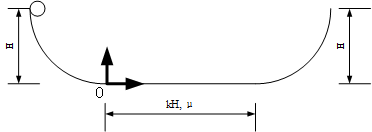
\includegraphics[width=0.5\textwidth]{../../resources/T0001.png}
    \caption{正则项的几何意义}
    \label{fig:1}
\end{figure*}

